\documentclass{beamer}

% Theme selection
\usetheme{Madrid}
\usecolortheme{default}

% Packages
\usepackage[utf8]{inputenc}
\usepackage{graphicx}
\usepackage{amsmath}
\usepackage{amssymb}
\usepackage{hyperref}
\usepackage{tikz}
\usetikzlibrary{shapes,arrows.meta,positioning}

% Title page information
\title[S2S Translation]{Speech to Speech Translation Systems}
\subtitle{Benchmarking and Implementation}
\author[Tanay, Jay, Kshitij, Vatsal]{Tanay Bhat  (22B3303) \\ Jay Mehta (22B1281) \\ Kshitij Vaidya (22B1829) \\ Vatsal Melwani (22B0396)}
\institute[IITB]{IIT Bombay}
\date{\today}

\begin{document}

% Title slide
\begin{frame}
\titlepage
\end{frame}

% Table of contents
\begin{frame}{Outline}
\tableofcontents
\end{frame}

% Introduction Section
\section{Introduction}

\begin{frame}{Introduction}
A usual S2S (speech-to-speech) pipeline consists of 3 main components - ASR (Automatic Speech Recognition), MT (Machine Translation) and TTS (Text-to-Speech). The ASR module converts the input speech into text, the MT module translates the text from source to target language and the TTS module converts the translated text back into speech. 
\newline

Previously, each stage was implemented separately and trained over different datasets. However, this leads to error propagation and information loss across the stages. Current state-of-the-art systems implement the complete pipeline as a unified system. This allows for better retention of prosodic and acoustic features across the stages, leading to more natural and accurate translations.
\end{frame}

% ASR Section
\section{Automatic Speech Recognition (ASR)}

\begin{frame}{ASR: Overview}
The ASR module of a S2S pipeline first converts the input speech into text. It involves several key components:
\begin{itemize}
    \item \textbf{Audio Preprocessing:} Noise reduction and feature extraction using MFCCs, Mel spectrograms etc.
    \item \textbf{Encoder:} Responsible for capturing temporal dependencies and contextual information of the input audio using the extracted features. Typically implemented using RNNs, CNNs, or Transformers.
    \item \textbf{Decoder:} Generates the output text sequence based on the encoder reprensentation. Current state-of-the-art models often use attention mechanisms to focus on relevant parts of the input during decoding.
\end{itemize}
\end{frame}

\begin{frame}{ASR Benchmarking: Setup}
We run our benchmarking on the LibriSpeech dataset from which 100 samples of english speech (around 8 minutes of audio). The audio signals are resampled to 16 kHz and normalised to be all lowercase and without punctuation. The following models are evaluated:
\begin{itemize}
    \item \textbf{OpenAI Whisper - Tiny:} Around 39M parameters
    \item \textbf{OpenAI Whisper - Base:} Around 74M parameters
    \item \textbf{OpenAI Whisper - Small:} Around 244M parameters
    \item \textbf{Distill Whisper - Small:} Around 166M parameters
    \item \textbf{OpenAI Whisper - Medium:} Around 394M parameters
\end{itemize}

We use word error rate (WER), character error rate (CER), sentence error rate (SER) and real-time factor (RTF) as our evaluation metrics.
\end{frame}

\begin{frame}{ASR Benchmarking: WER Results}
\begin{figure}
    \centering
    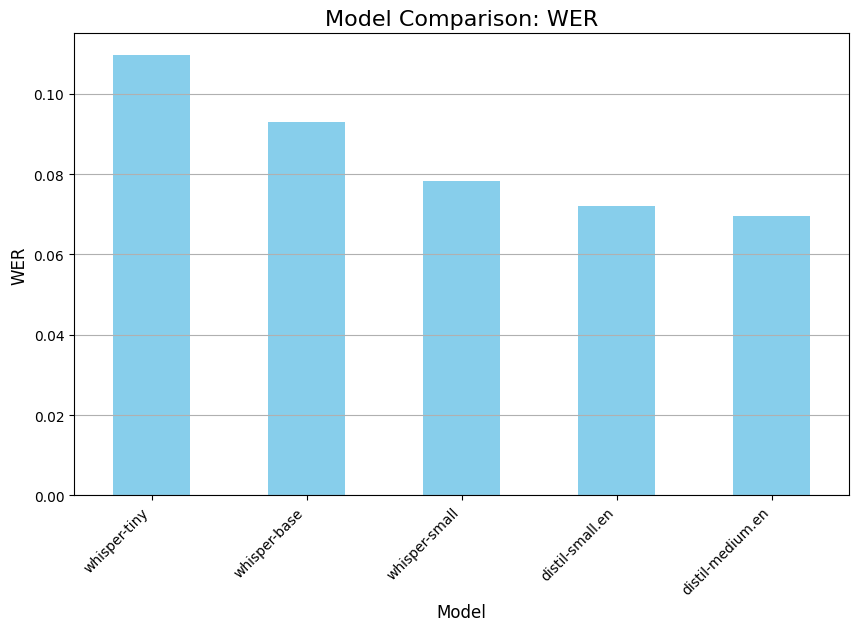
\includegraphics[width=0.75\textwidth]{Graphs/ASR_WER.png}
    \caption{WER results for different ASR models}
\end{figure}
\end{frame}

\begin{frame}{ASR Benchmarking: CER Results}
\begin{figure}
    \centering
    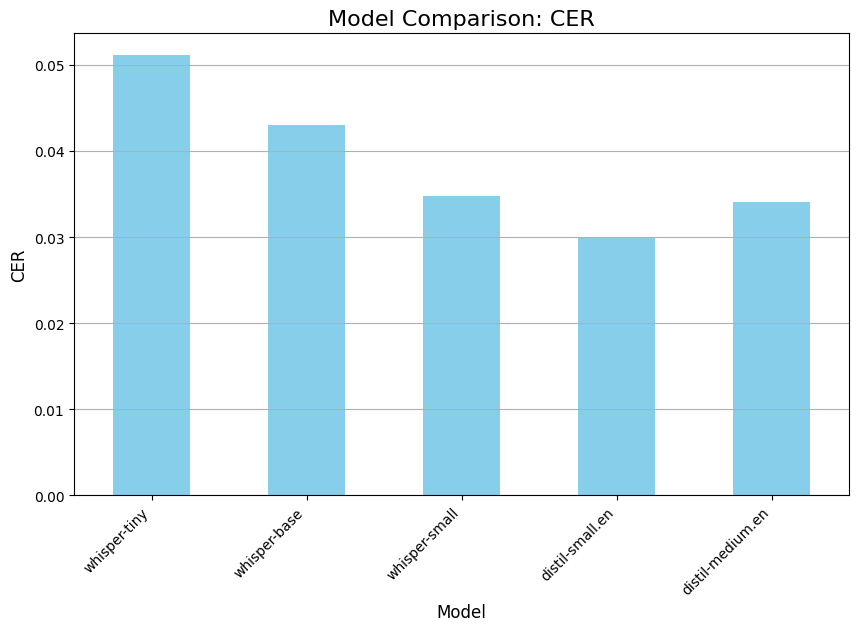
\includegraphics[width=0.75\textwidth]{Graphs/ASR_CER.png}
    \caption{CER results for different ASR models}
\end{figure}
\end{frame}

\begin{frame}{ASR Benchmarking: SER Results}
\begin{figure}
    \centering
    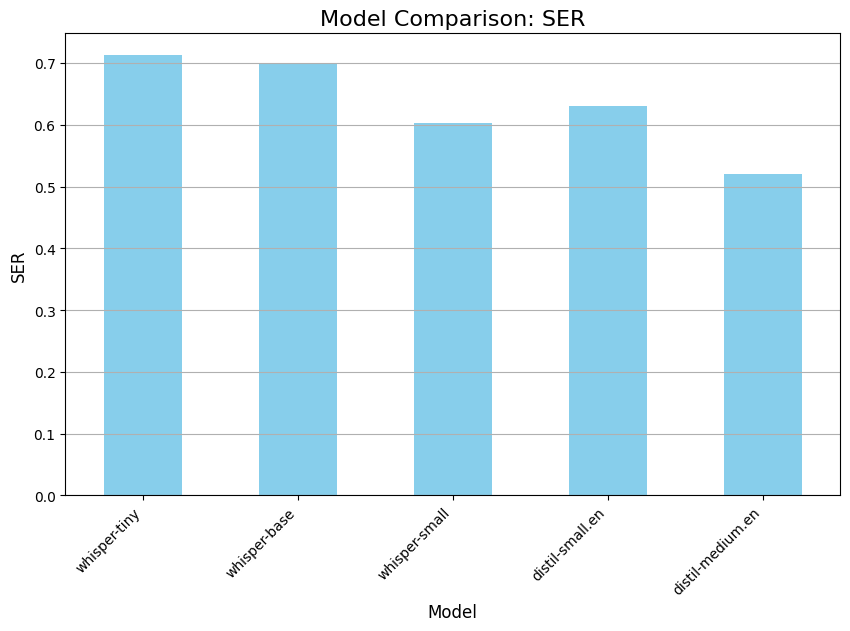
\includegraphics[width=0.75\textwidth]{Graphs/ASR_SER.png}
    \caption{SER results for different ASR models}
\end{figure}
\end{frame}

\begin{frame}{ASR Benchmarking: RTF Results}
\begin{figure}
    \centering
    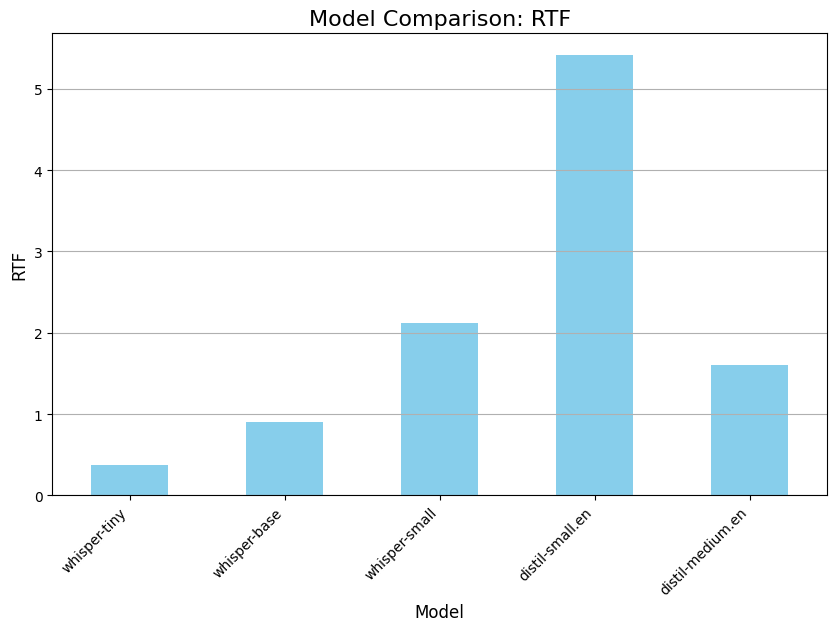
\includegraphics[width=0.75\textwidth]{Graphs/ASR_RTF.png}
    \caption{RTF results for different ASR models}
\end{figure}
\end{frame}

\begin{frame}{ASR Benchmarking: Inferences}
\begin{itemize}
\item Clear improvement in WER with increasing model size, with the medium model achieving the lowest WER of close to 0.07. The Distill small model performs better than OpenAI base model despite having fewer parameters.
\item CER shows similar trends however the Distill medium model performs slightly worse.
\item All models perform similary in terms of SER, with the Distill medium model performing the best.
\item Distill small has the worst RTF. This is an anomalous result as the Distill medium performs much better with the same running conditions. 
\end{itemize}
\end{frame}

% MT Section
\section{Machine Translation (MT)}

\begin{frame}{MT: Overview}
\begin{itemize}
\item Translates text from source to target language
\item Evolution: Rule-based → Statistical → Neural
\item Transformer architecture revolution
\item Quality assessment and evaluation
\end{itemize}
\end{frame}

\begin{frame}{MT: Key Approaches}
\begin{itemize}
\item Neural Machine Translation (NMT)
\item Transfer learning and multilingual models
\item Low-resource language handling
\item Context-aware translation
\end{itemize}
\end{frame}

% TTS Section
\section{Text-to-Speech (TTS)}
\begin{frame}{What is Text-to-Speech (TTS)?}
  \textbf{Text-to-Speech (TTS)} is the artificial synthesis of human-sounding speech from raw text.
  \vspace{0.5cm}
  
  \begin{itemize}
      \setlength\itemsep{1em}
      \item \textbf{Core Objectives:} 
      \begin{itemize}
          \item \textit{Intelligibility:} Clear, understandable pronunciation of words.
          \item \textit{Naturalness:} Accurate prosody, intonation, rhythm, and emotion.
      \end{itemize}
      
      \item \textbf{Evolution of the Technology:}
      \begin{itemize}
          \item \textbf{Concatenative (1990s-2000s):} Splicing together tiny fragments of pre-recorded human speech. Highly intelligible but sounded robotic and rigid.
          \item \textbf{Parametric (2000s-2010s):} Statistical models (like HMMs) generating audio based on parameters. Smoother, but sounded muffled or "buzzy".
          \item \textbf{Neural (Present):} Deep learning models predicting high-fidelity audio waves directly from text, achieving near-human naturalness.
      \end{itemize}
  \end{itemize}
\end{frame}

% Slide 2: The Block Diagram
\begin{frame}{The Standard Neural TTS Pipeline}
  \centering
  
  % Updated TikZ Block Diagram with smaller nodes
  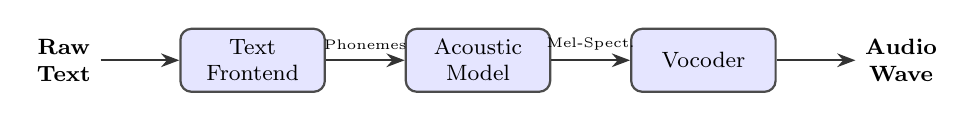
\begin{tikzpicture}[
      node distance=0.5cm and 1.0cm, % Reduced spacing between nodes
      block/.style={
          rectangle, 
          draw=black!70, 
          fill=blue!10, 
          thick, 
          text width=1.6cm,       % Reduced width
          align=center, 
          rounded corners, 
          minimum height=0.8cm,   % Reduced height
          font=\footnotesize      % Smaller font inside the blocks
      },
      arrow/.style={-{Stealth[scale=1.0]}, thick, draw=black!80}
  ]
      % Nodes
      \node (text) [font=\footnotesize\bfseries, align=center] {Raw\\Text};
      \node (frontend) [block, right=of text] {Text\\Frontend};
      \node (acoustic) [block, right=of frontend] {Acoustic\\Model};
      \node (vocoder) [block, right=of acoustic] {Vocoder};
      \node (audio) [font=\footnotesize\bfseries, align=center, right=of vocoder] {Audio\\Wave};

      % Arrows with labels
      \draw [arrow] (text) -- (frontend);
      \draw [arrow] (frontend) -- node[above, font=\tiny, align=center] {Phonemes} (acoustic);
      \draw [arrow] (acoustic) -- node[above, font=\tiny, align=center] {Mel-Spect.} (vocoder);
      \draw [arrow] (vocoder) -- (audio);
  \end{tikzpicture}
  
  \vspace{1.0cm}
  
  % Explanation Bullet Points
  \begin{itemize}
      \setlength\itemsep{0.5em}
      \item \textbf{Text Frontend:} Cleans and normalizes text (e.g., expanding "180" to "one hundred eighty") and performs Grapheme-to-Phoneme (G2P) conversion to determine pronunciation.
      \item \textbf{Acoustic Model:} Maps phonemes to acoustic representations, predicting pitch, energy, and duration. \textit{(Examples: Tacotron 2, FastSpeech)}
      \item \textbf{Vocoder:} Reconstructs the actual time-domain audio waveform from the highly compressed Mel-spectrogram. \textit{(Examples: WaveNet, HiFi-GAN)}
  \end{itemize}
\end{frame}
% \begin{frame}{TTS: Overview}
% \begin{itemize}
% \item Converts text into natural-sounding speech
% \item Components: Text analysis, prosody generation, synthesis
% \item Neural TTS models (WaveNet, Tacotron)
% \item Voice cloning and personalization
% \end{itemize}
% \end{frame}
\begin{frame}{Systems Under Evaluation}
    \vspace{0.3cm}
    
    % 3-Column Layout for Side-by-Side Comparison
    \begin{columns}[t]
        
        % Column 1: MMS-TTS
        \begin{column}{0.32\textwidth}
            \begin{block}{\small \centering \textbf{MMS-TTS}}
                % \vspace{0.1cm}
                \begin{itemize}\footnotesize
                    \setlength\itemsep{0.5em}
                    \item \textbf{Architecture:} VITS-based (End-to-End).
                    % \item \textbf{Core Feature:} Massive multilinguality (supports 1,100+ languages).
                    \item \textbf{Primary Strength:} Highly lightweight and efficient; state-of-the-art for low-resource languages.
                    \item \textbf{Limitation:} Generally single-speaker per model with fixed prosody.
                \end{itemize}
                \vspace{0.2cm}
            \end{block}
        \end{column}

        % Column 2: Parler-TTS
        \begin{column}{0.32\textwidth}
            \begin{block}{\centering \textbf{Parler-TTS}}
                % \vspace{0.1cm}
                \begin{itemize}\footnotesize
                    \setlength\itemsep{0.5em}
                    \item \textbf{Architecture:} Autoregressive Transformer.
                    % \item \textbf{Core Feature:} Text-promptable voice styling.
                    \item \textbf{Primary Strength:} Granular control over emotion, tone, pacing, and background noise via text descriptions.
                    \item \textbf{Limitation:} Higher inference latency due to autoregressive generation.
                \end{itemize}
                \vspace{0.2cm}
            \end{block}
        \end{column}

        % Column 3: XTTS-v2
        \begin{column}{0.32\textwidth}
            \begin{block}{\centering \textbf{XTTS-v2}}
                % \vspace{0.1cm}
                \begin{itemize}\footnotesize
                    \setlength\itemsep{0.5em}
                    \item \textbf{Architecture:} GPT-style + Mel/HiFi-GAN.
                    % \item \textbf{Core Feature:} Zero-shot voice cloning.
                    \item \textbf{Primary Strength:} Requires only $\sim$3 seconds of reference audio; supports cross-lingual voice cloning.
                    \item \textbf{Limitation:} High resource consumption compared to non-autoregressive models.
                \end{itemize}
                \vspace{0.2cm}
            \end{block}
        \end{column}

    \end{columns}
    
    \vspace{0.5cm}
    
    % Summary takeaway at the bottom
    \begin{center}
        \textit{\small These systems represent three distinct TTS paradigms: \textbf{Scale} (MMS), \textbf{Promptability} (Parler), and \textbf{Cloning} (XTTS).}
    \end{center}
    
\end{frame}

\begin{frame}{Evaluation Metrics for TTS Models}
    \vspace{0.1cm}
    
    \begin{columns}[T]
        
        % Column 1: Intelligibility & Speed
        \begin{column}{0.48\textwidth}
            \begin{block}{Intelligibility \& Efficiency}
                \begin{itemize}\small
                    \setlength\itemsep{0.5em}
                    \item \textbf{Word Error Rate (WER)} \\
                          \textit{What it is:} Transcription accuracy of the audio using an ASR system. Lower is better. \\
                        %   \textbf{[\textcolor{red}{$\downarrow$} Lower is Better]}
                          
                    \item \textbf{Character Error Rate (CER)} \\
                          \textit{What it is:} Similar to WER, but captures finer phonetic/spelling errors. Lower is better.\\
                        %   \textbf{[\textcolor{red}{$\downarrow$} Lower is Better]}
                          
                    \item \textbf{Real-Time Factor (RTF)} \\
                          \textit{What it is:} Processing time divided by generated audio length. Lower is better. \\
                        %   \textbf{[\textcolor{red}{$\downarrow$} Lower is Better]}
                \end{itemize}
            \end{block}
        \end{column}

        % Column 2: Prosody & Acoustics
        \begin{column}{0.48\textwidth}
            \begin{block}{Prosody \& Expressiveness}
                \begin{itemize}\small
                    \setlength\itemsep{0.3em}
                    \item \textbf{Pitch Variance ($F_0$ Std Dev)} \\
                          \textit{What it is:} Range of intonation. \\
                        %   \textbf{[\textcolor{blue}{$\approx$} Target Match is Better]}
                          
                    \item \textbf{Energy Dynamics (RMS Std)} \\
                          \textit{What it is:} Variations in volume/loudness. \\
                        %   \textbf{[\textcolor{blue}{$\approx$} Target Match is Better]}
                          
                    \item \textbf{Speaking Rate} \\
                          \textit{What it is:} Speed (Syllables/words per sec). \\
                        %   \textbf{[\textcolor{blue}{$\approx$} Target Match is Better]}
                          
                    \item \textbf{Pause Ratio (Onset/s)} \\
                          \textit{What it is:} Frequency of breath/silence pauses. \\
                        %   \textbf{[\textcolor{blue}{$\approx$} Target Match is Better]}
                \end{itemize}
            \end{block}
        \end{column}

    \end{columns}
    
    % \vspace{0.4cm}
    
    % Crucial Clarification Note
    % \begin{center}
        % \footnotesize{\textit{\textbf{*Note on Prosodic Metrics:} Unlike WER or RTF, acoustic metrics do not strictly benefit from being "maximized." The goal is to minimize the distance to the \textbf{Ground Truth} human audio. Too low results in robotic, flat speech; too high results in unnatural, exaggerated speech.}}
    % \end{center}
    
\end{frame}

\begin{frame}{TTS: Benchmarking Results}
    \begin{table}[]
    \centering
    \begin{tabular}{c|c|c|c|c}
        \textbf{Model} & \textbf{Language} & \textbf{Latency (ms)} & \textbf{RTF} & \textbf{Throughput (cps)} \\
        \hline
        MMS-TTS & English & 2621.382 & 0.439 & 31.711 \\
        MMS-TTS & Hindi & 2451.2891 & 0.432 & 27.49 \\
        Parler-TTS & English & 68026.311 & 11.264 & 1.281 \\
        XTTS-v2 & English & 26182.9 & 3.438 & 3.491 \\
        XTTS-v2 & Hindi & 23687.88 & 3.204 & 2.718 \\
    \end{tabular}
    \caption{Benchmarking results for TTS models across Performance Metrics.}
    \end{table}

\end{frame}

\begin{frame}{TTS: Benchmarking Results}
    \begin{table}[]
    \centering
    \begin{tabular}{c|c|c|c}
        \textbf{Model} & \textbf{Language} & \textbf{WER} & \textbf{CER} \\
        \hline
        MMS-TTS & English & 34.892 & 17.968\\
        MMS-TTS & Hindi & - & -\\
        Parler-TTS & English & 27.57 & 19.854\\
        XTTS-v2 & English & 20.465 & 6.825\\
        XTTS-v2 & Hindi & - & -\\    
    \end{tabular}
    \caption{Benchmarking results for TTS models across Performance Metrics (Contd.).}
    \end{table}

    \footnotesize{\textit{*WER/CER for Hindi were turning out to be extremely high due to ASR model's poor performance on Hindi audio, so we have omitted those values to avoid skewing the analysis.}}
\end{frame}

\begin{frame}{TTS: Benchmarking Results}
    \begin{table}[]
    \centering
    \begin{tabular}{c|c|c|c|c}
        \textbf{Model} & \textbf{Language} & \textbf{Pitch (Mean)} & \textbf{Pitch (Std)} & \textbf{Pitch Range} \\
        \hline
        MMS-TTS & English & 99.978 & 19.158 & 81.388 \\
        MMS-TTS & Hindi & 148.216 & 37.359 & 176.392 \\
        Parler-TTS & English & 233.055 & 54.52 & 253.809 \\

        XTTS-v2 & English & 141.029 & 29.674 & 136.078 \\

        XTTS-v2 & Hindi & 139.625 & 16.915 & 76.358\\    
    \end{tabular}
    \caption{Benchmarking results for TTS models across Prosodic Metrics (Contd.).}
    \end{table}
\end{frame}


\begin{frame}{TTS: Benchmarking Results}
    \begin{table}[]
    \centering
    \begin{tabular}{c|c|p{2cm}|p{2cm}|p{2cm}}
        \textbf{Model} & \textbf{Language} & \textbf{Speaking Rate} & \textbf{Energy Dynamics} & \textbf{Pause Ratio} \\
        \hline
        MMS-TTS & English & 6.788 & 0.067 & 0.183 \\
        MMS-TTS & Hindi & 5.808 & 0.093 & 0.246 \\
        Parler-TTS & English & 5.35 & 0.082 & 0.153 \\
        XTTS-v2 & English & 4.284 & 0.099 & 0.212 \\

        XTTS-v2 & Hindi & 4.268 & 0.1002 & 0.186 \\    
    \end{tabular}
    \caption{Benchmarking results for TTS models across Prosodic Metrics.}
    \end{table}
\end{frame}

\begin{frame}{TTS: Plots}
    \begin{figure}
        \centering
        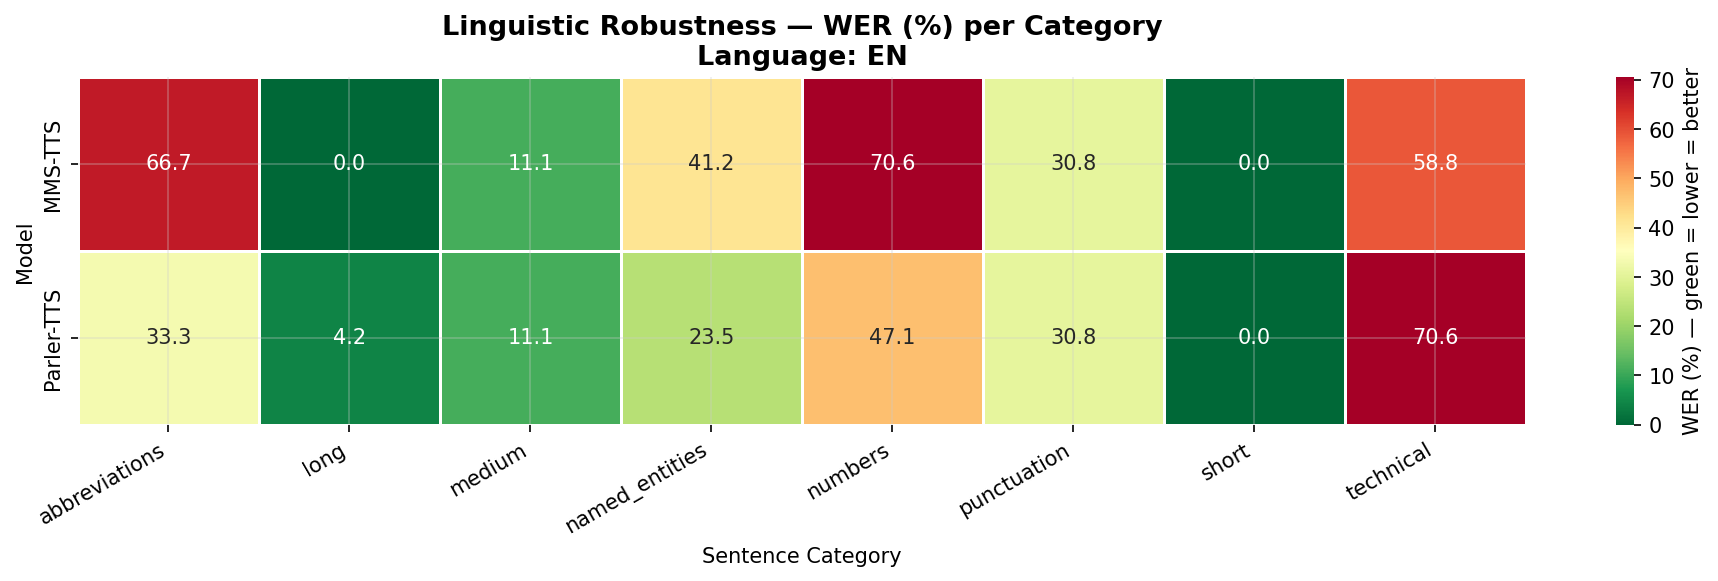
\includegraphics[width=0.6\textwidth]{Graphs/04_robustness_heatmap_en.png}
        \caption{WER Heatmap for English for MMS-TTS and Parler-TTS for different types of sentences.}
    \end{figure}
    \begin{figure}
        \centering
        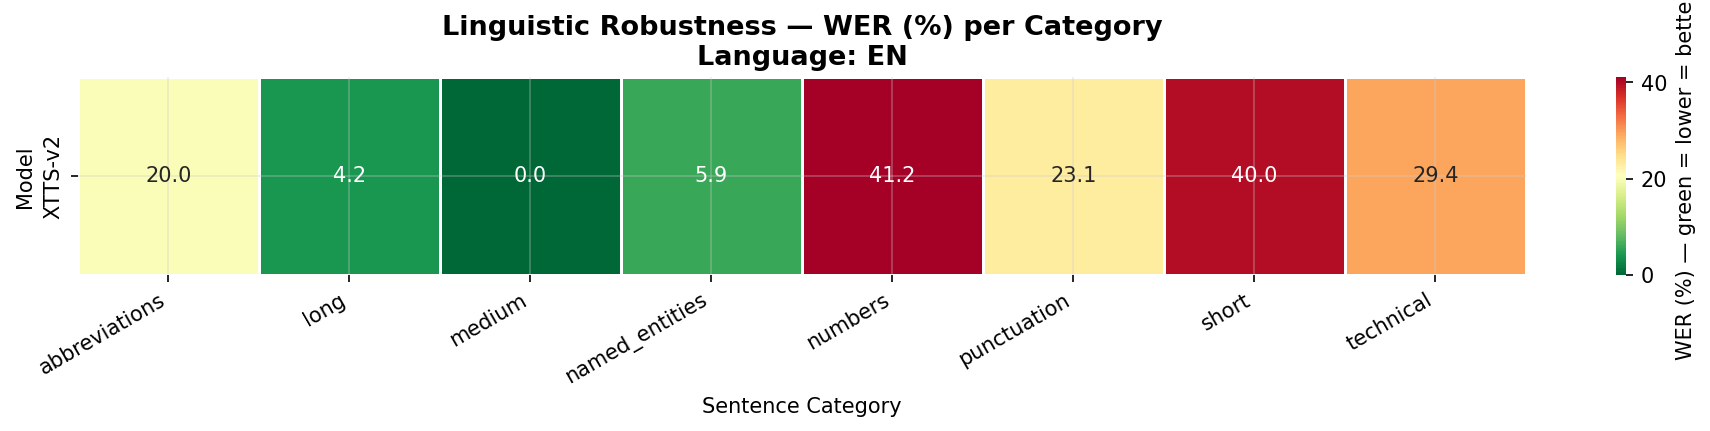
\includegraphics[width=0.6\textwidth]{Graphs/04_robustness_heatmap_en_2.png}
        \caption{WER Heatmap for English for XTTS-v2 for different types of sentences.}
    \end{figure}
\end{frame}

% Full Pipeline Section
\section{Full Pipeline Integration}

\begin{frame}{End-to-End Pipeline}
We also implemented a full S2S pipeline using few of the models that we benchmarked here and compared them against the existing SeamlessM4T-V2 (2.3B parameters) model. The models that we used for the pipeline were:
\begin{itemize}
\item \textbf{ASR:} OpenAI Whisper - Base (74M parameters)
\item \textbf{MT:} Helsinki-NLP Opus-MT (English to Hindi) (77M parameters)
\item \textbf{TTS:} MMS-TTS by Meta AI (559M parameters)
\end{itemize}
\end{frame}

\begin{frame}{S2S pipeline: Scoring Metrics}
We use the following scoring metrics for the end-to-end pipeline:
\begin{itemize}
\item \textbf{METEOR:} Measure n-gram precision and recall while accounting for synonyms and stemming.
\item \textbf{chrF++:} Extends character n-gram F-score with word-level n-grams, capturing both fine-grained and coarse-grained translation quality.
\item \textbf{RTF:} Real-time factor, measuring the speed of the system relative to real-time processing.
\item \textbf{Latency:} Time taken for the system to process and respond to input.
\item TODO : add prosodic metrics for the end-to-end pipeline as well
\end{itemize}
\end{frame}

\begin{frame}{S2S pipeline: Results}
TODO add graphs
\end{frame}

% Conclusion Section
\section{Conclusion}

\begin{frame}{Conclusion}
\begin{itemize}
\item Integrated ASR-MT-TTS systems enable powerful applications
\item Continued advances in neural architectures
\item Challenges remain in low-resource scenarios
\item Future directions: multimodal integration, personalization
\end{itemize}
\end{frame}

\begin{frame}{Thank You}
\begin{center}
{\Large Thank you for your attention!}

\vspace{1cm}

Questions?

\vspace{1cm}

\small
Contact: your.email@example.com
\end{center}
\end{frame}

\end{document}